\chapter[绪论]{绪\qquad论}
\section{研究背景与意义}
近年来,随着信息技术的快速发展,互联网所产生和处理的数据量也在迅猛增长。有研究表明,过去两年内产生的数据量已经占世界数据总量的 $90\%$\cite{bradshaw2013big}。因此,如何存储这些数据成为了存储系统相关研究的核心问题之一。传统上的集中式存储系统采用计算能力和 I/O 能力强悍的大型主机进行数据存储,然而对于 PB 量级甚至更高的数据量\cite{li2013erasure},传统的集中式存储由于过高的设计和维护成本渐渐难以满足日益增长的存储需求。在目前的数据中心中,普遍采用大量的性价比更高的小型主机,通过分布式文件系统协同存储数据中心中的海量数据,其中常见的分布式文件系统有 Hadoop 分布式文件系统(Hadoop Distributed File System,即 HDFS)\cite{shvachko2010hadoop}和 Ceph 分布式文件系统\cite{weil2006ceph}等,其架构如图 \ref{p9} 所示。在此背景下,如何在分布式文件系统中进行高效且可靠的数据存储,是目前存储领域研究的热点。

\begin{figure}[!htb]
\centering
\resizebox{.8\textwidth}{!}{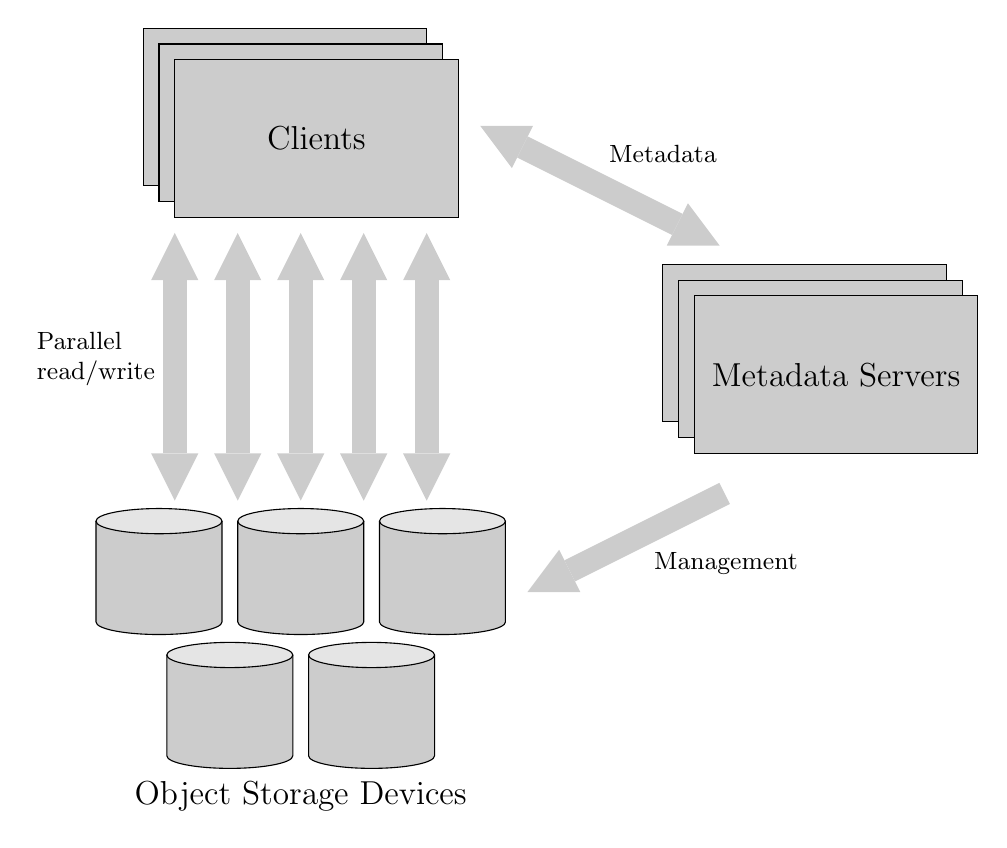
\begin{tikzpicture}
\fill [color=white,opacity=0] (0, 0) rectangle (12, 10);

\newcommand\cylinder[3]{%
\fill [color=black!20!white] (#2-#1, #3-.8*#1) arc (180:360:#1 and .2*#1) -- (#2+#1, #3+.8*#1) arc (0:-180:#1 and .2*#1) -- cycle;%
\filldraw [fill=black!10!white] (#2, #3+.8*#1) ellipse (#1 and .2*#1);%
\draw (#2-#1, #3+.8*#1) -- (#2-#1, #3-.8*#1) arc (180:360:#1 and .2*#1) -- (#2+#1, #3+.8*#1);%
}
\cylinder{.8}{2.5}{1.4}
\cylinder{.8}{4.3}{1.4}
\cylinder{.8}{1.6}{3.1}
\cylinder{.8}{3.4}{3.1}
\cylinder{.8}{5.2}{3.1}
\node at (3.4, .25) [font=\fontsize{12pt}{20pt}\selectfont] {Object Storage Devices};
\filldraw [fill=black!20!white] (1.4, 8) rectangle (5, 10);
\filldraw [fill=black!20!white] (1.6, 7.8) rectangle (5.2, 9.8);
\filldraw [fill=black!20!white] (1.8, 7.6) rectangle (5.4, 9.6);
\node at (3.6, 8.6) [font=\fontsize{12pt}{20pt}\selectfont] {Clients};
\filldraw [fill=black!20!white] (8, 5) rectangle (11.6, 7);
\filldraw [fill=black!20!white] (8.2, 4.8) rectangle (11.8, 6.8);
\filldraw [fill=black!20!white] (8.4, 4.6) rectangle (12, 6.6);
\node at (10.2, 5.6) [font=\fontsize{12pt}{20pt}\selectfont] {Metadata Servers};
\newcommand\clienttoosd[1]{%
\fill [color=black!20!white] (#1-.15, 4.6) rectangle (#1+.15, 6.8);%
\fill [color=black!20!white] (#1-.3, 6.8) -- (#1, 7.4) -- (#1+.3, 6.8) -- cycle;%
\fill [color=black!20!white] (#1-.3, 4.6) -- (#1, 4) -- (#1+.3, 4.6) -- cycle;%
}
\clienttoosd{1.8}
\clienttoosd{2.6}
\clienttoosd{3.4}
\clienttoosd{4.2}
\clienttoosd{5}
\node at (.8, 5.8) [align=left,font=\fontsize{9pt}{10.8pt}\selectfont] {Parallel\\read/write};
\fill [rotate around={63.435:(7.2,8)},color=black!20!white] (7.05, 6.9) rectangle (7.35, 9.1);
\fill [rotate around={63.435:(7.2,8)},color=black!20!white] (6.9, 9.1) -- (7.2, 9.7) -- (7.5, 9.1) -- cycle;
\fill [rotate around={63.435:(7.2,8)},color=black!20!white] (6.9, 6.9) -- (7.2, 6.3) -- (7.5, 6.9) -- cycle;
\node at (8, 8.4) [font=\fontsize{9pt}{10.8pt}\selectfont] {Metadata};

\fill [rotate around={-63.435:(7.8,3.6)},color=black!20!white] (7.65, 2.5) rectangle (7.95, 4.7);
\fill [rotate around={-63.435:(7.8,3.6)},color=black!20!white] (7.5, 2.5) -- (7.8, 1.9) -- (8.1, 2.5) -- cycle;
\node at (8.8, 3.2) [font=\fontsize{9pt}{10.8pt}\selectfont] {Management};
\end{tikzpicture}
}
\caption{常见的分布式对象存储系统架构图}
\label{p9}
\end{figure}

对于这些分布式存储系统来说,由于系统由大量的存储节点共同组成,其中每个节点均为不可靠的小型主机,因此发生存储节点故障是不可避免的。那么如何在部分节点发生故障之后,保证分布式存储系统仍能够继续提供服务,并且有效地进行故障恢复,则是分布式存储系统研究中需要解决的重要问题之一。目前常用的分布式存储系统一般采用多副本备份技术来作为存储系统的容错性设计,但由于多副本备份技术引入了大量的数据冗余,导致数据的存储成本也被大大提高。近年来,有学者将纠删码技术应用于分布式存储系统的设计中\cite{chen2017ahdfs,xie2019az,wei2018new,haddock2017gpu,drucker2018comeback,li2019openec},以期在保障系统容错性的同时,通过数学计算大幅度减少恢复数据需要的冗余备份数据量。这些研究通过更好地使用纠删码进行数据的冗余备份存储,从而大大降低数据的冗余度,节约存储成本。

然而由于纠删码需要对一个数据块整体进行计算、备份与恢复,因此在数据块进行修改时,需要对整个块进行解码并重新编码,导致系统性能难以提高。因此,在目前的分布式文件系统中,纠删码的使用主要还是倾向于假设文件极少修改,或者文件内容修改的效率并不是分布式存储引擎主要优化目标。比如在 Ceph 等最新的分布式文件系统中,其纠删码引擎虽然实现了对象的修改,然而由于其直接将对象的修改操作映射为数据块的修改操作,因此在纠删码引擎上进行对象修改操作是较为低效的。然而,在分布式数据库或实时流计算等领域若应用此类存储系统,会导致性能急剧下降。故难以使用统一的存储结构实现分布式文件系统、分布式数据库系统和分布式流存储系统等各种不同类型的分布式存储系统。在此基础上,对于基于纠删码实现的对象存储引擎中数据的高效修改算法的研究,可以使基于纠删码的分布式存储系统能够更广泛地应用于不同存储领域,有利于在更多领域减少数据冗余备份所带来的额外开销。
\section{主要研究内容与贡献}
本文在调研并了解当前已有的文件分布式文件系统和纠删码最新研究成果的基础上,研究了基于纠删码和对象存储的分布式存储系统,旨在进一步提高分布式存储系统的存储效率。当前基于纠删码的分布式存储系统在通用的对象存储上取得了不错的效果,然而在数据冗余度和对数据块的修改优化等方面还存在着一定的提升空间。针对大数据时代不断增长的存储需求,降低数据冗余可以减少数据备份所需要的存储介质数量,大幅降低数据的存储成本。针对数据库、实时流计算等对数据修改和附加要求更高的存储需求,优化数据修改算法能使更多类型的存储系统可以通过采用纠删码的方式来减少存储冗余。本文基于动态纠删码编码策略实现了一个统一支持对象存储和文件存储的分布式存储系统如图 \ref{p2} 所示。此系统分为基于动态纠删码编码策略的对象存储和基于对象存储的文件存储两大部分,下面将依次简要进行介绍。

\begin{figure}[!htb]
\centering
\resizebox{.8\textwidth}{!}{\begin{tikzpicture}
\fill [color=white,opacity=0] (0, 0) rectangle (12, 4);

\draw [dashed,rounded corners] (0, 0) rectangle (1.8, 1);
\node at (0.9, 0.5) [align=center,font=\fontsize{9pt}{10.8pt}\selectfont] {存储设备\\速度};
\draw [dashed,rounded corners] (0, 1.5) rectangle (1.8, 2.5);
\node at (0.9, 2) [align=center,font=\fontsize{9pt}{10.8pt}\selectfont] {存储设备\\可靠性};
\draw [dashed,rounded corners] (0, 3) rectangle (1.8, 4);
\node at (0.9, 3.5) [font=\fontsize{9pt}{10.8pt}\selectfont] {对象可用性};
\draw [dashed,rounded corners] (2.55, 1.5) rectangle (4.35, 2.5);
\node at (3.45, 2) [align=center,font=\fontsize{9pt}{10.8pt}\selectfont] {纠删码\\编码策略};
\draw [rounded corners] (5.1, 1.5) rectangle (6.9, 2.5);
\node at (6, 2) [font=\fontsize{9pt}{10.8pt}\selectfont] {对象存储};
\draw [rounded corners] (7.65, 0.5) rectangle (9.45, 1.5);
\node at (8.55, 1) [font=\fontsize{9pt}{10.8pt}\selectfont] {块存储};
\draw [rounded corners] (7.65, 2.5) rectangle (9.45, 3.5);
\node at (8.55, 3) [font=\fontsize{9pt}{10.8pt}\selectfont] {文件存储};
\draw [rounded corners] (10.2, 1.5) rectangle (12, 2.5);
\node at (11.1, 2) [font=\fontsize{9pt}{10.8pt}\selectfont] {数据库存储};

\draw [dashed] (1.8, 0.5) -- (2.55, 2);
\draw [dashed] (1.8, 2) -- (2.55, 2);
\draw [dashed] (1.8, 3.5) -- (2.55, 2);
\draw [dashed] (4.35, 2) -- (5.1, 2);

\draw [-latex] (7.65, 3) -- (6.9, 2);
\draw [-latex] (7.65, 1) -- (6.9, 2);
\draw [-latex] (10.2, 2) -- (6.9, 2);
\draw [-latex] (10.2, 2) -- (9.45, 3);
\draw [-latex] (10.2, 2) -- (9.45, 1);
\end{tikzpicture}
}
\caption{基于纠删码对象存储的分布式文件系统设计}
\label{p2}
\end{figure}

本文首先实现了一个基于动态纠删码编码策略的对象存储系统。纠删码编码技术不同于多副本备份技术,它无需重复存储多份相同的原始数据,而是将原始数据分为 $n$ 个原始数据单元,并通过纠删码编码计算,增加额外的 $m$ 个冗余数据单元,通过这 $n+m$ 个原始数据单元和冗余数据单元中的任意至少 $n$ 个数据单元,均可通过计算还原出原始数据。即基于 $n+m$ 个数据单元的纠删码的编码方案,最多可以容忍 $m$ 个数据单元失效。然而在数据中心中,由于存储的数据量是不断变化的,因此分布式文件系统中的节点会动态地进行增加或者替换,这些增加或替换的存储介质的型号和批次往往不尽相同。因此,在分布式文件系统中,每一个节点之间的速度和可靠性也是有差异的。面对非一致速度和可靠性的节点,我们若采用传统的固定原始数据单元和冗余数据单元数量的方式计算纠删码编码,则会忽略节点之间的这些差异信息,从而难以得到最优的存储性能。同时,不同类型的文件根据其重要性的不同,也有着不同的可用性需求。因此,如果能充分利用待存储对象的可用性以及存储设备的可靠性等信息,来动态地确定纠删码的编码方案,则可以提高系统中存储设备的利用率,进而提升系统的整体性能,并降低存储成本。本文提出了 On-demand ARECS 算法(On-demand Availability and Reliability Oriented Adaptive Erasure Coded Storage System),其综合存储设备的类型、批次和使用状况等信息,对存储设备的可靠性进行预测,进而对存储于设备上的数据可靠性进行推断,并依据对象数据自身的可用性需求,动态地确定纠删码存储策略,并根据各个节点的实时状态计算得出满足可用性需求的最快节点集合,从而选取当前状况下存储速度最快的存储节点,解决了慢速节点的瓶颈问题,从而兼顾了存储效率和存储可靠性,实现了基于动态非一致存储设备可靠性和数据可用性的自适应纠删码对象存储系统。

在上述自适应纠删码对象存储系统的基础上,针对数据可能频繁地进行修改和附加的特点,我们研究了基于纠删码编码的数据修改算法。该算法将文件修改和附加操作的函数调用抽象为修改事件对象,并将修改事件对象单独存储于对象存储系统中。通过定义修改事件对象,我们将文件的随机修改和附加转化为对象的新增操作,从而避免了纠删码的解码与重新编码,大幅降低了基于纠删码的分布式存储系统的额外开销,一定程度上提升了基于纠删码实现的存储引擎的文件存储性能。对于并发执行的文件修改和附加操作,我们采用了一个无锁的修改事件队列,从而避免了并发修改和附加时文件锁的开销,从而支持高并发的分布式文件系统操作。针对频繁修改的对象,本文提出在系统空闲时间进行修改事件整合的方法,从而解决过多的修改事件带来的读取性能损失。

本文相较于已有的分布式文件系统,针对非一致的对象可用性和存储设备可靠性灵活地定义纠删码策略,并针对存储设备的实时速度和可用性动态进行存储池规划和存储节点选择,从而高效地利用存储节点,降低数据冗余。针对基于纠删码的分布式文件系统的数据修改问题,本文提出了将文件修改和附加操作抽象为修改事件对象进行存储的算法,实现了无锁的高效并发写入,扩展了基于纠删码的分布式文件系统的应用场景。

\section{本文组织结构}
本文的主要内容分为以下六个章节:

第一章为绪论。本章首先介绍了本文的研究背景与研究意义,面对不断增长的存储需求,分布式存储系统渐渐替代了传统的集中式存储系统。为了兼顾数据的安全性和存储效率,在分布式文件系统中,常采用纠删码进行数据的冗余备份。在此基础上,简要概括了本文的主要研究内容与贡献,提出了一种针对非一致的存储设备可靠性和数据可用性进行纠删码编码的策略,从而提高基于纠删码的分布式存储系统的存储效率,并介绍了一种将文件修改和附加操作抽象为修改事件的方案,从而解决基于纠删码的存储系统在数据修改时需要解码和重新编码的效率问题。最后,介绍了本文的组织结构。

第二章为相关工作。本章首先介绍了目前存储系统中数据可能发生丢失的几种可能原因,并分别介绍了目前主流存储系统中的数据备份与恢复算法,其中存储利用率最高的备份与恢复算法便是基于纠删码的存储算法。之后,梳理了当前存储系统中使用的三类主流纠删码编码方案:阵列码、低密度奇偶校验码和里德-所罗门码。里德-所罗门码是唯一的可以使用任意原始数据单元个数和冗余数据单元个数的 MDS 编码(即存储效率达到理论上的最优),但是其存在着一定的计算开销。最后,总结了目前主流分布式文件系统中基于里德-所罗门码纠删码编码引擎的实现方案和数据修改算法。针对基于里德-所罗门码纠删码的计算效率问题,介绍了目前几种分布式存储系统中里德-所罗门码计算优化的最新研究成果。针对基于里德-所罗门码纠删码编码的存储系统在数据修改时解码和重新编码的性能开销问题,总结了目前分布式文件系统中针对文件存储结构的最新研究成果。

第三章为基于非一致可靠性存储的数据可用性评估策略。本章介绍了 On-demand ARECS 算法中存储设备可靠性和数据可用性的推断部分。针对不同重要性的数据,我们需要选取适当的数据可用性来达到更高的成本收益率。针对实际分布式存储系统中存储设备类型、批次和使用状况等特征,提出了一种对存储设备的可靠性进行动态估计的方法,并基于此存储设备的可靠性对其上存储的数据可用性进行估计,从而保证满足设定的数据可用性。针对实际存储系统中损坏节点的会被定期更换和重建的特点,我们在模型中引入了数据重建时间,从而保证存储系统在动态条件下能够满足数据所需的可用性。最后,本章对 On-demand ARECS 算法的磁盘故障率模型和成本收益模型进行了模拟实验验证。

第四章为面向动态数据可用性的纠删码对象存储策略。本章介绍了 On-demand ARECS 算法中的存储节点选择部分。根据数据本身的可用性需求以及基于存储设备推断的数据可用性保障,通过分析节点实时性能数据,最小化存储时所需要的读写时间,从而选取最优的存储设备组合,实现自适应的对象存储系统。针对过大的对象若直接进行纠删码计算时编码矩阵过大,导致计算开销过高的问题,我们通过数据分块的方式进行纠删码的计算,并假设各数据块大小均等,从而计算模型中的数据读写时间,保证存储系统高效地进行大文件的读写。最后,本章在开源的 Tahoe-LAFS 分布式文件系统上实现了基于 On-demand ARECS 算法的动态纠删码对象存储系统,对 On-demand ARECS 算法的存储效率和存储速度进行了实验验证。

第五章为基于纠删码对象存储的分布式文件存储。本章首先介绍了基于 On-demand ARECS 算法进行纠删码编码的对象存储系统的设计和物理存储组织方式,并通过 FUSE 技术设计了一种基于自适应对象存储的分布式文件系统中间件。其次,针对基于纠删码编码的对象存储在数据修改时需要解码并重新编码,导致数据修改开销过大的特点,我们将文件的修改和附加操作抽象为修改事件,存储于只读的对象存储系统中。为了保证并发状态下数据修改的效率,我们应用了基于数组的无锁队列来处理修改事件队列。针对数据多次修改后可能导致的读取速度减慢问题,我们提出了一种在系统空闲时间对文件修改对象进行合并的策略。最后,我们在基于 Tahoe-LAFS 的分布式文件系统上对此算法的文件修改和附加操作性能进行了测试。

第六章为结论与展望。本章首先回顾了全文的工作,介绍了基于 On-demand ARECS 算法和文件修改事件对象算法的分布式文件系统对存储速度进行的优化。之后,总结了目前基于纠删码的分布式文件系统研究中的热点和挑战,并针对数据损坏时的数据重建、纠删码编码和解码的开销和磁盘故障率的有效估计等问题展望了未来可能的研究方向。
